%% chapter 4

\chapter{基于SCENIC的GRN推断}
  SCENIC是一种利用单细胞RNA测序数据同时进行基因调节网络重建和细胞状态识别的计算方法。SCNEIC能够帮助我们从基因表达矩阵中鉴定转录因子和细胞状态,提供驱动细胞异质性机制的重要生物学见解。

\section{SCENIC算法原理}
  SCENIC的工作流程主要有3步:GRNBoost2,基于共表达确定潜在的TF靶标;RcisTarget,进行TF基序富集分析并确定直接的靶标(调节子);AUCell,用于对单个细胞上调节子(或其他基因集)的活性进行评分。下面我们将对每一步算法原理进行介绍。

\begin{figure}[!htb]
  \centering
  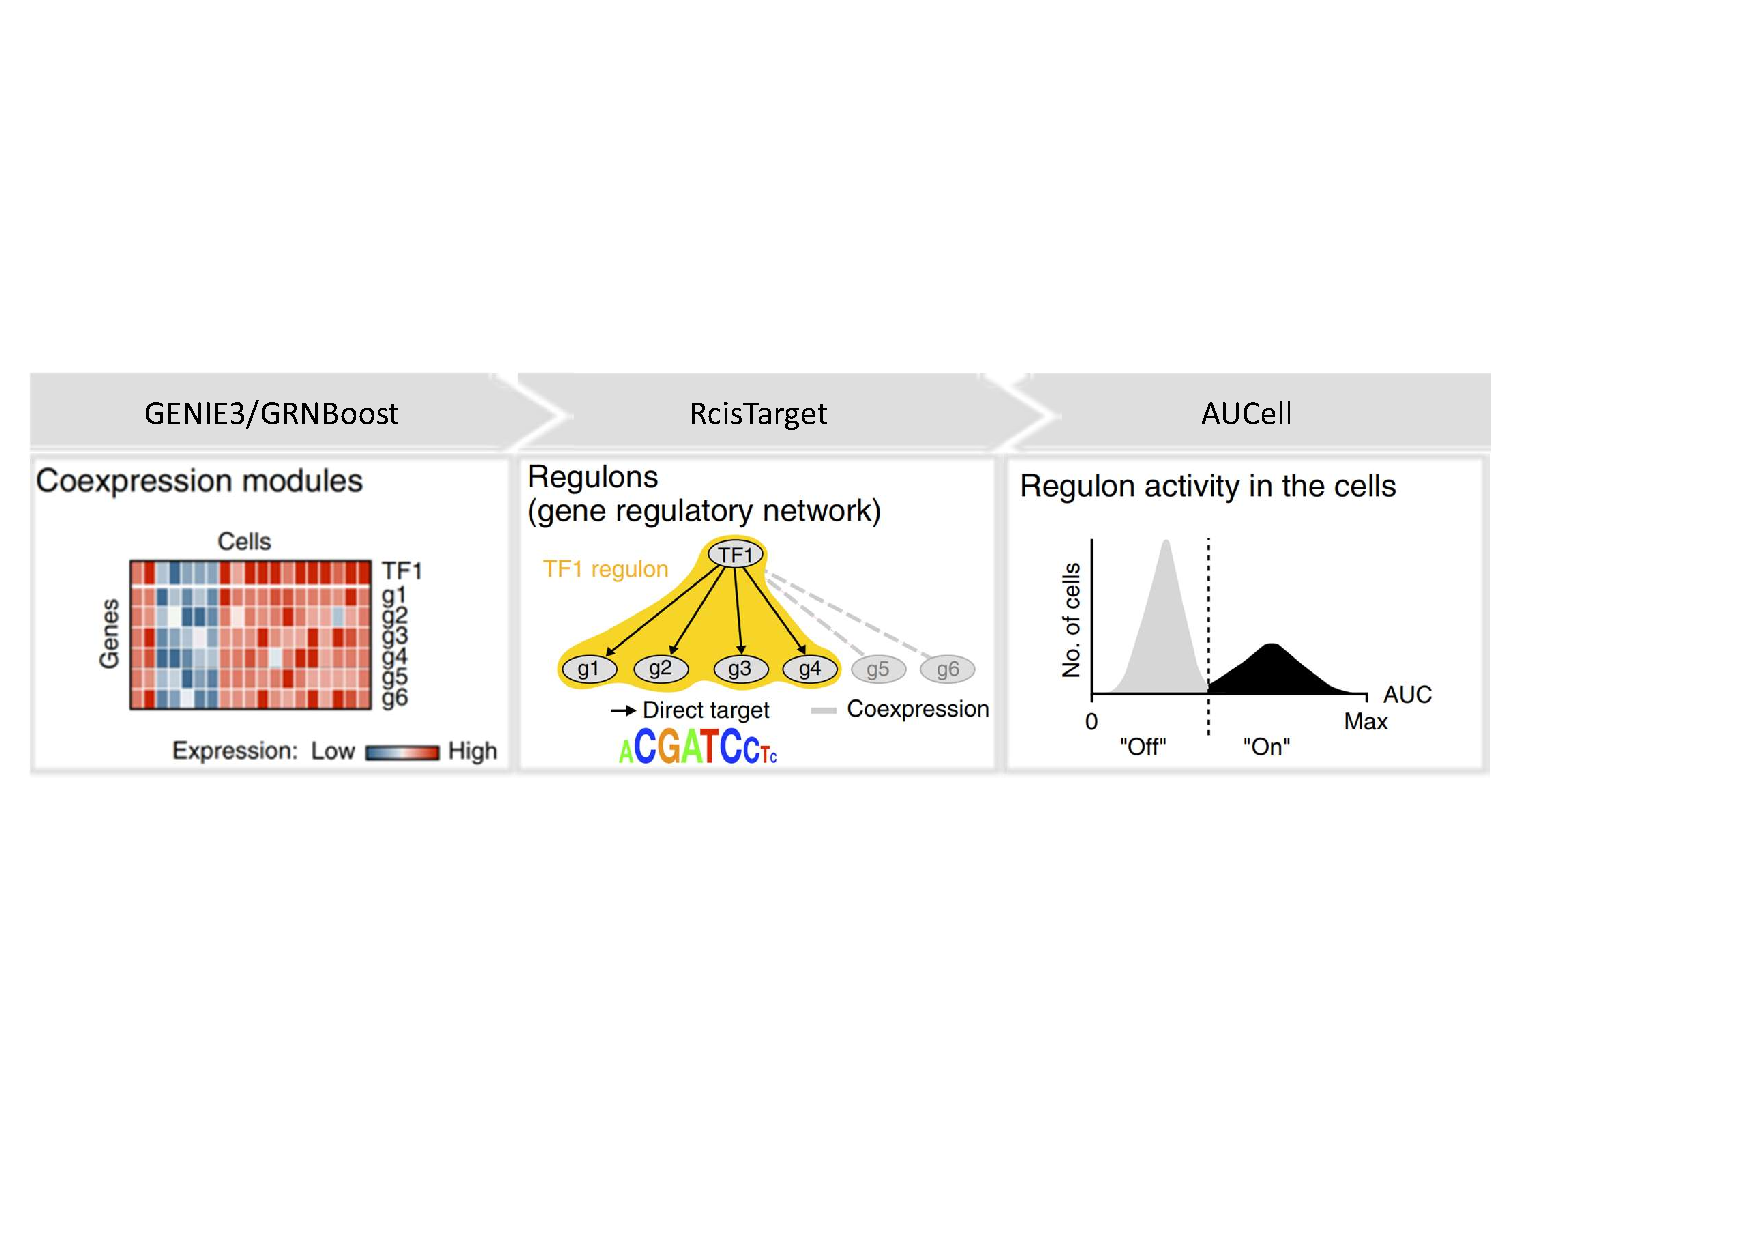
\includegraphics[width=0.8\textwidth]{figs/scenic-workflow.pdf}
  \caption{SCENIC算法流程}
  \label{fig:scenic-workflow}
\end{figure}

\subsection{GRNBoost2}
  像GENIE3\cite{huynh2010inferring}一样,GRNBoost2属于基于回归的GRN推理方法\cite{sanguinetti2019gene}。对于数据集中的每个基因,使用一组候选转录因子(TF)的表达值对基于树的回归模型进行训练,以预测其表达谱。每个模型都会产生部分GRN,并具有从最佳预测TF到目标基因的调控关联。将所有调控关联组合在一起,并按重要性排序,以最终确定GRN的输出。

  Gradient-Boosting Machines(GBM)\cite{friedman2001greedy}是GRNBoost2\cite{moerman2019grnboost2}部分的核心。GBM是一种用于回归和分类问题的机器学习技术,它以一组弱预测模型(通常为决策树)的形式生成预测模型。当决策树是弱学习者时,结果算法称为梯度提升树,通常胜过随机森林。

  GBM的算法原理与梯度下降类似:梯度下降是在参数空间中寻找一个最优点,而GBM则是在函数空间(或者说我们设定的函数集合)寻找一个最优函数。在最优化函数的过程中,我们需要一个优化目标,这通常通过设定损失函数来实现。

  在许多有监督的学习问题中,一个输出变量$y$和一个输入向量$x$通过联合概率分布$P(x,y)$来描述。使用已知$x$和对应$y$所构成的训练集$\{(x_{1},y_{1}),...,(x_{n},y_{n})\}$,目标是找到函数$F(x)$的近似值$\hat{F}(x)$。该近似值应最小化某些指定损失函数$L(y,F(x))$的期望值:
\begin{equation}
  \hat{F} = \mathop{\arg\min}_{F}\mathbb{E}_{x,y}[L(y,F(x))]
\end{equation}

  GBM假设真实值为$y$,并在某些类$\mathcal{H}$中利用函数$h_{i}(x)$的加权和寻求其的近似值$\hat{F}(x)$,这被称为基学习器:
\begin{equation}
  \hat{F}(x) = \sum^{M}_{i=1}\gamma_{i}h_{i}(x) + const
\end{equation}

  根据经验风险最小化原理,该方法尝试找到一个近似值$\hat{F}(x)$,该函数将在训练集计算的损失函数平均值最小化,即最小化经验风险。这一过程是从一个由常数函数$F_{0}(x)$组成的模型开始的,然后以贪心算法的过程逐步扩展它:
\begin{equation}
  F_{0}(x) = \mathop{\arg\min}_{\gamma}\sum^{n}_{i=1}L(y_{i},\gamma)
\end{equation}
\begin{equation}
  F_{m}(x) = F_{m-1}(x) + \mathop{\arg\min}_{h_{m}\in{\mathcal{H}}}\left[\sum^{n}_{i=1}L(y_{i},F_{m-1}(x_{i}) + h_{m}(x_{i}))\right]
\end{equation}
这里,$h_{m}\in{\mathcal{H}}$是一个基学习器函数。

  但上面这个过程是在计算上不可行的优化问题,GBM便将其进一步简化。这个想法便是对这个最小化问题(功能梯度下降)应用最陡峭的下降步骤。如果我们考虑连续的情况,也就是说,$\mathcal{H}$在$\mathbb{R}$上是任意微分函数的集合,我们将根据以下方程式更新模型:
\begin{equation}
  F_{m}(x) = F_{m-1}(x) - \gamma\sum^{n}_{i=1}{\nabla}_{F_{m-1}}L(y_{i},F_{m-1}(x_{i}))
\end{equation}
\begin{equation}
  {\gamma}_{m} = \mathop{\arg\min}_{\gamma}\sum^{n}_{i=1}L(y_{i},F_{m-1}(x_{i}) - \gamma{\nabla}_{F_{m-1}}L(y_{i},F_{m-1}(x_{i})))
\end{equation}
这里,微分是对函数$F_{i}(i\in\{1,...,m\})$所计算的来的,$\gamma$是步长。但是,在离散情况下,即当集合$\mathcal{H}$只有有限个元素时,我们选择最接近$L$梯度的候选函数$h$,然后可以根据上述等式通过线搜索来为其计算系数$\gamma$。但这种方法是一种启发式的方法,无法给出给定问题的精确解决方案,只能提供一个近似的解,其伪代码如算法\ref{alg:gbm}所示。

\begin{algorithm}[H]
  \caption{Gradient-Boosting Machine}
  \SetAlgoLined
  \KwIn{training set $\{(x_{i},y_{i})\}^{n}_{i=1}$, a differentiable loss function $L(y,F(x))$, number of iterations $M$}
  \KwOut{$F_{M}(x)$}
  Initialize model with a constant value: $$F_{0}(x) = \mathop{\arg\min}_{\gamma}\sum^{n}_{i=1}L(y_{i},\gamma)$$\\
  \For{$m\leftarrow 1$ \KwTo $M$}{
    Compute so-called pseudo-residuals: $$r_{im} = -\left[\frac{\partial L(y_{i},F(x_{i}))}{\partial F(x_{i})}\right] for i=1,...,n$$\\
    Fit a base learner(e.g. tree) $h_{m}(x)$ to pseudo-residuals, i.e. train it using the training set $\{(x_{i},r_{im})\}^{n}_{i=1}$.\\
    Compute multiplier ${\gamma}_{m}$ by solving the following one-dimensional optimization problem: $${\gamma}_{m} = \mathop{\arg\min}_{\gamma}\sum^{n}_{i=1}L(y_{i},F_{m-1}(x_{i}) + {\gamma}h_{m}(x_{i}))$$\\
    Update the model: $$F_{m}(x) = F_{m-1}(x) + {\gamma}_{m}h_{m}(x)$$\\
  }
  Return $F_{M}(x)$.\\
  \label{alg:gbm}
\end{algorithm}

\subsection{RcisTarget}
  RcisTarget可为基因列表识别富集的TF结合基序和候选转录因子。简而言之,RcisTarget基于两个步骤。首先,它选择在基因组中的基因转录起始位点(TSS)的周围环境中显着过量表达的DNA基序。这是通过在数据库中应用基于恢复的方法来实现的,该数据库包含每个基序的全基因组跨物种排名。保留了注释为相应TF并获得归一化富集得分(NES)> 3.0的基序。接下来,对于每个基序和基因组,RcisTarget预测候选目标基因(即,基因组中排在最前沿的基因)。该方法基于Aerts等人\cite{aerts2010robust}描述的方法,该方法也可以在i-cisTarget(网络界面)\cite{herrmann2012cistarget}和iRegulon(Cytoscape插件)\cite{verfaillie2014iregulon}中实现。因此,当使用相同的参数和数据库时,RcisTarget可提供与i-cisTarget或iRegulon相同的结果,并以Janky等人\cite{verfaillie2014iregulon}中的其他TFBS富集工具为基准。
\subsection{AUCell}
  AUCell可帮助研究人员在单细胞RNA测序数据中鉴定具有活跃基因调控网络的细胞。AUCell的输入是一个基因集,输出是每个细胞中“活跃”的基因集。在SCENIC中,这些基因集是调控子,由TF及其推定的靶标组成。

  AUCell会计算跨越特定细胞中所有基因排名的恢复曲线下的区域,并将其作为调节子的富集程度,从而根据该表达值对它们进行排名。然后,AUCell使用AUC来计算输入基因集的关键子集是否在每个细胞的排名顶部都得到了富集。通过这种方式,AUC代表了基因签名中表达基因的比例及其与细胞内其他基因相比的相对表达值。

\section{选择SCENIC算法的原因}
  由于细胞的状态是受基因调节子调控的,其内部是一个十分复杂的调控网络。我们应当考虑这种潜在的调节网络,以获取更加生物合理的细胞状态定义,因为它对于我们总结结论有着重要的参考作用。我们希望选择的GRN推断算法应具备以下优势:
\begin{itemize}
  \item 聚类结果应与细胞真实的种类有着较好的匹配度,即较高的调整兰德指数(ARI)。
  \item 所推断的GRN应具备较高鲁棒性,即数据集大小不会对检测出的转录因子有很大影响。
  \item 具有较低的算法复杂度,对于大数据集仍可以在较短的时间内完成基因调控网络推断。
\end{itemize}

  作为最新提出的GRN推断算法SCENIC,具备以上的所有优势。Aibar在其2017年的工作\cite{aibar2017scenic}中就以上标准与以往的GRN推断算法进行了比较。为了测试SCENIC算法的性能,Aibar使用一个公开的人为标注数据集作为基线,统计所有GRN推断方法所得到聚类结果的ARI。其中,ARI定义如下:
\begin{equation}
  ARI = \frac{{\sum}_{ij}\binom{n_{ij}}{2} - \frac{\left[{\sum}_{i}\binom{a_{i}}{2}{\sum}_{j}\binom{b_{j}}{2}\right]}{\binom{n}{2}}}{\frac{1}{2}\left[{\sum}_{i}\binom{a_{i}}{2}+{\sum}_{j}\binom{b_{j}}{2}\right]-\frac{\left[{\sum}_{i}\binom{a_{i}}{2}{\sum}_{j}\binom{b_{j}}{2}\right]}{\binom{n}{2}}}
\end{equation}
其中,设$X_{i}(i\in{1,...,r})$表示真实类别,$Y_{j}(j\in{1,...,s})$表示预测类别,则式中$n_{ij}$表示本属于$X_{i}$类被预测为$Y_{j}$类数据的数量,$a_{i}$表示数据集中属于$X_{i}$类数据的数量,$b_{j}$表示数据集中被预测为$Y_{j}$类数据的数量。由其统计结果(图\ref{fig:scenic-prt}a)可见,SCENIC算法的聚类结果相比其它GRN推断算法得到的结果更为精确。

  为了测试SCENIC算法的鲁棒性,Aibar在比较性能时使用的数据集中随机抽取100个数据组成一个较小的数据集。其将各种GRN推断方法在原数据集发掘出的转录因子作为基线,统计小数据集上发掘出转录因子的召回率和准确率。尤其统计结果(图\ref{fig:scenic-prt}b)可见,SCENIC算法相比其它GRN推断算法具备较高的鲁棒性。

  最后,在对大数据集的处理效率方面,SCENIC算法中使用了GENIE3算法\cite{huynh2010inferring}更为高效的变体——GRNBoost2算法\cite{moerman2019grnboost2}。GRNBoost2基于与GENIE3相同的概念,纯粹从基因表达矩阵中推断每个靶基因的调节子。但是,GRNBoost2使用Gradient-Boosting Machines(GBM)\cite{friedman2001greedy}代替了随机森林模型。这种实现方式大大减少了推断GRN所需的时间(图\ref{fig:scenic-prt}c),并为在非常大的数据集上进行网络推断铺平道路。

\begin{figure}[!htb]
  \centering
  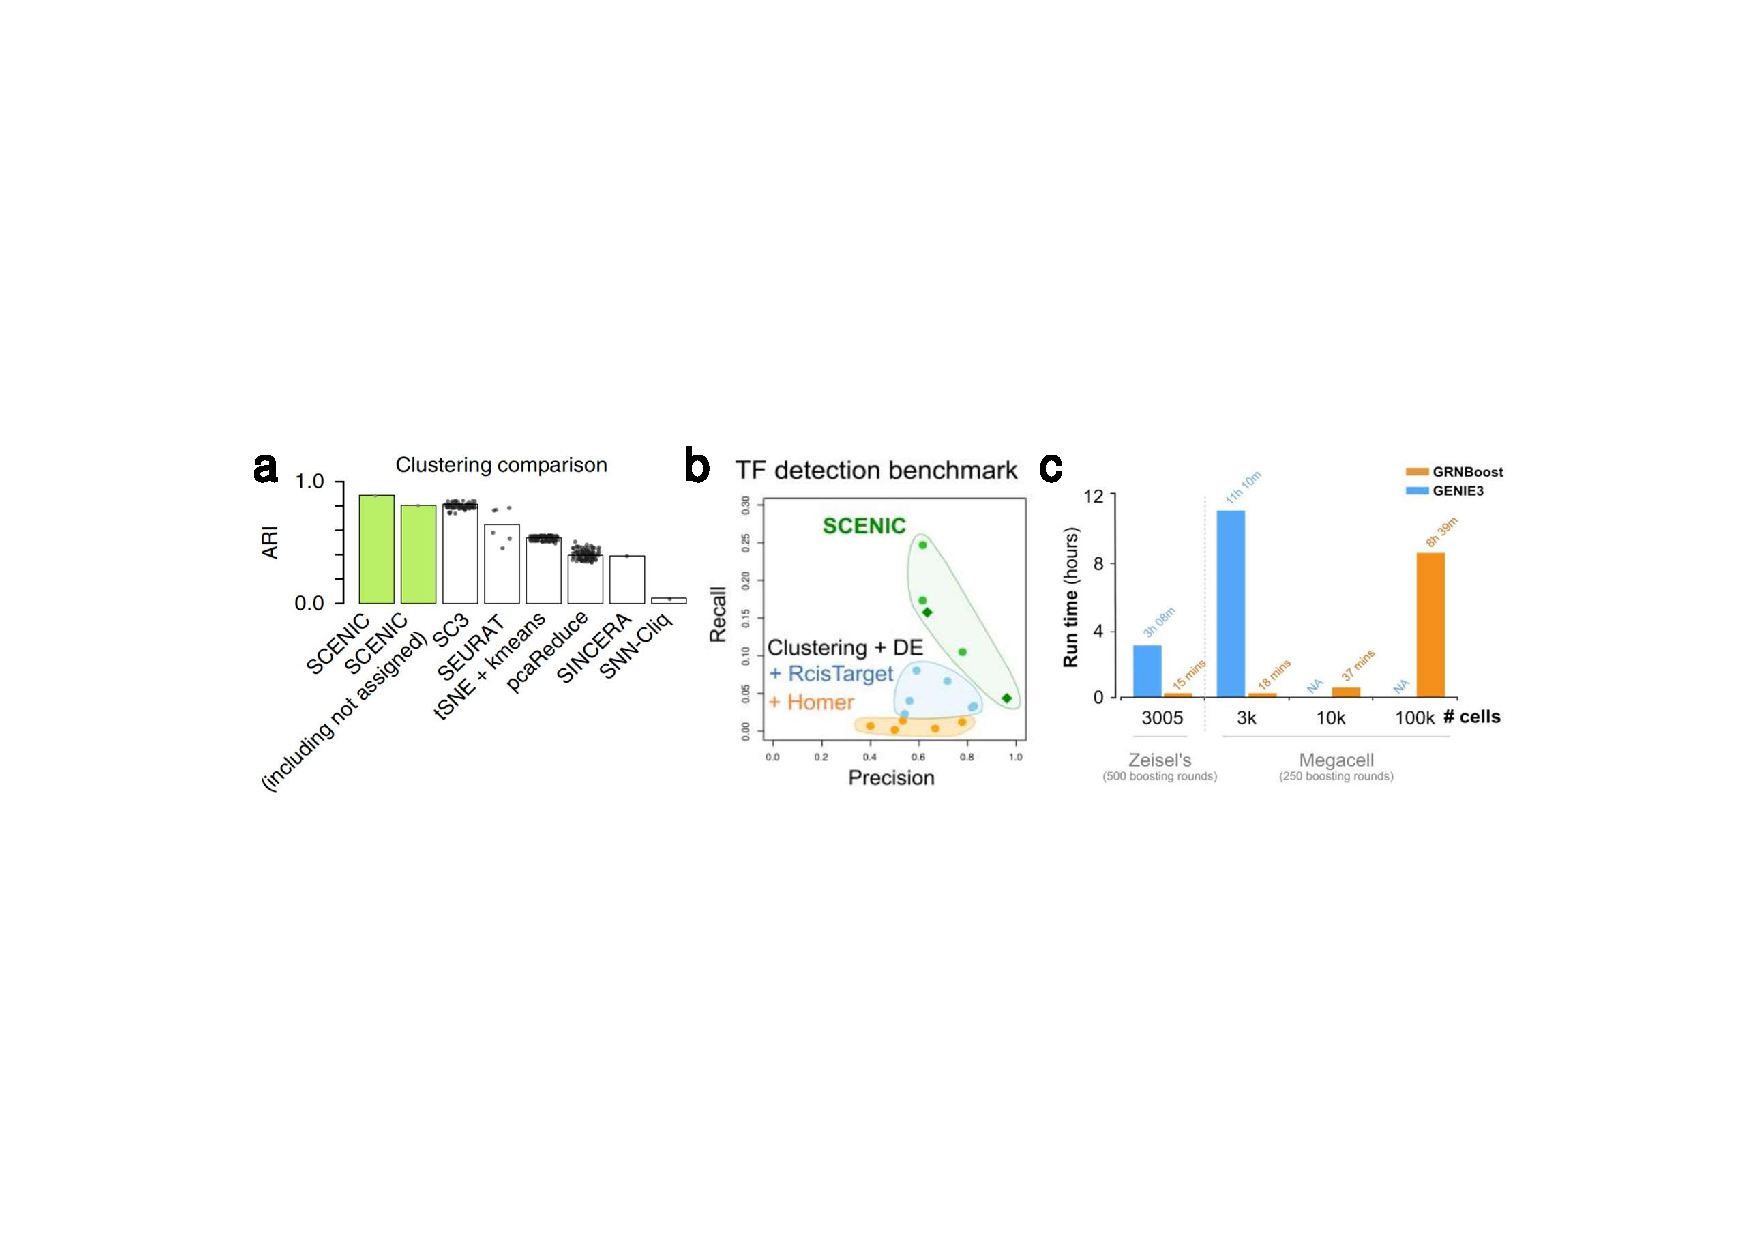
\includegraphics[width=0.8\textwidth]{figs/scenic-prt.pdf}
  \caption{SCENIC算法与其他GRN推断算法的比较}
  \label{fig:scenic-prt}
\end{figure}

